\documentclass[10pt]{beamer}

\usepackage[utf8]{inputenc}
% \AtBeginSection[]
% {
%   \begin{frame}
%     \frametitle{Table of Contents}
%     \tableofcontents[currentsection]
%   \end{frame}
% }
\usetheme{Berkeley}
\usepackage{mleftright}
\mleftright

\usepackage{tikzsymbols}

\newcommand{\abs}[1]{\left\lvert#1\right\rvert}
\newcommand{\norm}[1]{\left\lVert#1\right\rVert}
\renewcommand{\vec}[1]{\boldsymbol{#1}}
\newcommand{\proj}[2]{\operatorname{proj}_{#2}\left(#1\right)}
\newcommand{\dotprod}[2]{\left\langle#1,#2\right\rangle}
\newcommand{\compconj}[1]{\overline{#1}}
\newcommand{\T}{\mathrm{T}}
\newcommand{\set}[1]{\left\{#1\right\}}
\newcommand{\bigO}[1]{\mathcal{O}\left(#1\right)}
%Information to be included in the title page:

\title[COSC6364 Adv. Numerical Analysis] %optional
{COSC6364 Adv. Numerical Analysis}

\subtitle{Introduction}

\author[Wu, Panruo] % (optional, for multiple authors)
{P. ~Wu\inst{1}}

\institute[VFU] % (optional)
{
  \inst{1}%
  Computer Science\\
  University of Houston
  % \and
  % \inst{2}%
  % Faculty of Chemistry\\
  % Very Famous University
}

\date[Spring 2020] % (optional)
{Spring 2020}

\logo{
\includegraphics[height=0.5cm]{nsm-computer-science-primary.png}}

\begin{document}

\frame{\titlepage}

\begin{frame}
  \frametitle{Table of Contents}
  \tableofcontents
\end{frame}
\section{What is this course about?}
\begin{frame}
  \frametitle{What is this course about?}
  \begin{itemize}
    \item <2-> Basically two major parts:
    \begin{itemize}
      \item <3-> Numerical linear algebra (matrix computations)
      \item <4-> (Convex) optimization 
    \end{itemize}
    \item <5-> The topics are primarily geared towards (large scale) statistical learning (\alert{learning from data}) and to scientific/engineering computing (\alert{technical computing}).
  \end{itemize} 
\end{frame}

\section{Tentative Topics}
\subsection{Numerical Linear Algebra}
\begin{frame}
  \frametitle{Tentative Topics for Numerical Linear Algebra}
  \begin{itemize}
    \item <2-> Matrix multiplication, norms, orthogonality
    \item <3-> Singular value decomposition (SVD)
    \item <4-> QR factorization and least square problems
    \item <5-> LU/Cholesky factorization for linear systems
    \item <6-> QR algorithm and Eigenvalue Decomposition (EVD)
    \item <7-> Iterative methods for solving linear equation and eigen/singular decomposition
    \item <8-> Fast implementation, parallelization, randomization, etc...
  \end{itemize}
\end{frame}

\subsection*{Books}
\begin{frame}
  \frametitle{Books}
  \begin{columns}
    \column{0.5\textwidth}
    \begin{itemize}
      \item <2-> (Highly recommend; main reference) 
      
            Numerical Linear Algebra (Lloyd N. Trefethen, David Bau)

            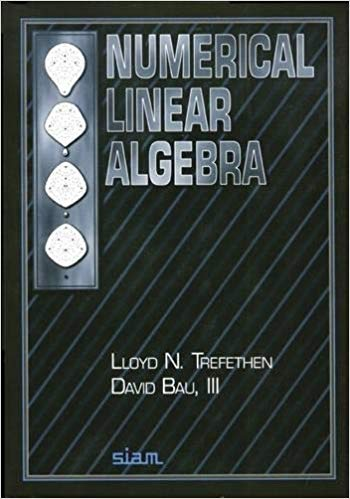
\includegraphics[height=0.5\textheight]{numerical-linear-algebra.jpg}
    \end{itemize}
    \column{0.5\textwidth}
    \begin{itemize}
      \item <3-> Scientific Computing: An introductory Survey (Michael T. Heath)
      
            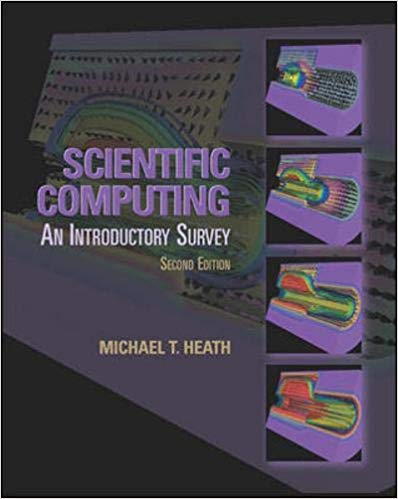
\includegraphics[height=0.5\textheight]{scientific-computing.jpg}
    \end{itemize}
  \end{columns}
\end{frame}

\subsection{Convex Optimization}
\begin{frame}[t]
  \frametitle{Tentative Topics for Convex Optimization}
  \begin{itemize}
   \item <2-> Convexity
   \item <3-> Gradient/subgradient descent, proximal GD, stochastic GD
   \item <4-> Duality, KKT conditions
   \item <5-> (Quasi) Newton methods, Interior point methods
   \item <6-> Coordinate descent, dual ascent, Alternating direction method of multipliers (ADMM), etc...
  \end{itemize}
\end{frame}

\subsection*{Books}
\begin{frame}
  \frametitle{Books}
  \begin{columns}
    \column{0.5\textwidth}
    \begin{itemize}
      \item <2-> (Highly recommend; main reference) 
      
            Numerical Linear Algebra (Lloyd N. Trefethen, David Bau)

            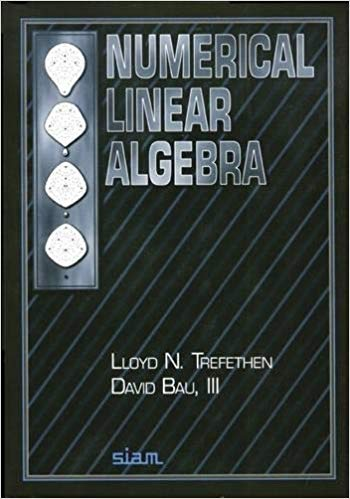
\includegraphics[height=0.5\textheight]{numerical-linear-algebra.jpg}
    \end{itemize}
    \column{0.5\textwidth}
    \begin{itemize}
      \item <3-> Scientific Computing: An introductory Survey (Michael T. Heath)
      
            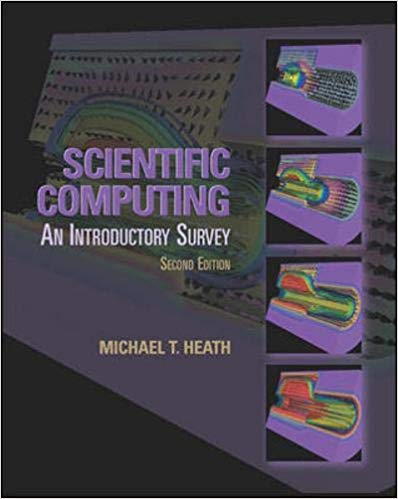
\includegraphics[height=0.5\textheight]{scientific-computing.jpg}
    \end{itemize}
  \end{columns}
\end{frame}

\section{Objectives}
\subsection{Numerical Linear Algebra}
\begin{frame}
  \frametitle{Objectives for Numerical Linear Algebra}
  Upon successful completion of this course, the students should be able to
  \begin{itemize}
    \item <2-> Understand basic matrix computation concepts and algorithms;
    \item <3-> Know how to compute matrix factorization/inversion, linear systems, least square problems, eigen/singular value decomposition, ...
    \item <4-> Analyze the computational cost of numerical algorithms
    \item <5-> Apply different algorithms for different situations; able to diagnose numerical stability and errors
  \end{itemize}
\end{frame}

\subsection{Optimization}
\begin{frame}
  \frametitle{Objectives for Optimization}
  Upon successful completion of this course, the students should be able to
  \begin{itemize}
    \item <2-> Recognize convex optimizations
    \item <3-> Be able to formulate and transform convex optimization problem
    \item <4-> Understand how different optimization algorithms work; under what conditions do they work; the convergence rate; the cost of each iteration.
    \item <5-> Use KKT conditions to solve/characterize optimization problem
    \item <6-> Understand the role of optimization in statistical learning
  \end{itemize}
\end{frame}

\section{Why study all these?}
\begin{frame}
  \frametitle{Why study all these?}
  \begin{itemize}
    \item <2-> Data science is largely about manipulating matrices/vectors.
    \item <3-> There are four aspects that are important for manipulating large matrices (which are not covered in typical college linear algebra courses):
    \begin{itemize}
      \item <4-> \alert{Speed}: big matrix can be very slow to compute.
        \begin{itemize}
          \item <5-> Doing pretty much anything interesting on dense matrix cost about \(\bigO{n^3}\) floating point operations; on a large matrix where \(n \approx 10^5\), \(n^3 \approx 10^{15}\) operations \(\approx\) 280 hours assuming \(10^9\) operations/s.
        \end{itemize}
      \item <6-> \alert{Accuracy}: digital computers do finite precision arithmetic, meaning that each arithmetic (usually) incurs some small error (rounding error). If you do billions of operations does the errors accumulate or amplify?
        \begin{itemize}
          \item <7-> Some algorithms are more stable than the others;
        \end{itemize}
      \item <8-> \alert{Memory}: the storage is usually \(\bigO{n^2}\); again grows fast with size of matrix.
      \item <9-> \alert{Scalability}: you don’t have enough memory space or computing power so you wantto use parallel computers. Does more nodes mean faster execution time?
      \end{itemize}
    \item <10-> Because the world is harsh, we’ll frequently need to tradeoff between them: but first you need to know and understand them
  \end{itemize}
\end{frame}

\section{Can’t I just use a library?}
\begin{frame}
  \frametitle{Can't I just use a library?}
  \ldots like Sci-kit learn / [put your favorite framework here]

  Probably, but what if
  \begin{itemize}
    \item <2-> Too slow
    \item <3-> Low quality result. What’s wrong?
    \item <4-> Variants not implemented (\Sadey)?
    \item <5-> Doing cutting edge research/development?
  \end{itemize}
  \onslide<6->{It’s worth knowing what’s going on under the hood. Plus, you get to study and play with really cool stuff that I found fascinating.}
\end{frame}
\end{document}
